% Chapter 4

\chapter{Análise e Desenho} % Main chapter title
\label{chap:Chapter4} % For referencing the chapter elsewhere, use \ref{chap:Chapter4} 

	Após a revisão da literatura, realizada no capítulo \ref{chap:Chapter2}, conseguimos chegar à conclusão que as ferramentas de \gls{LLM} quando utilizadas para correlação de incidentes, análise do histórico de \textit{tickets} e sugestões de mitigação, podem ajudar os membros das equipas de suporte a compreender melhor os incidentes e resolvê-los de uma forma mais eficaz e eficiente.
	
	Assim, a solução, através da integração com um \gls{LLM}, deve ser capaz de apoiar os \gls{OCEs} na interpretação, análise e mitigação dos incidentes. Esta solução é baseada, numa fase inicial, pela ligação entre o incidente a resolver e os registos anteriores, aumentando a informação do incidente atual numa linguagem percetível para qualquer membro da equipa de suporte, com mais ou menos experiência, e em qualquer contexto de trabalho e pressão. Com o apoio de integrações externas, como \textit{Confluence}, pretende-se também aumentar o contexto do serviço afetado de forma a indicar uma mitigação mais viável. Com a correlação de incidentes funcional e documentação dos próprios produtos, procura-se encontrar sugestões de mitigação para o utilizador que permitam uma rápida ação para resolver, temporariamente ou definitivamente, o problema, diminuindo o \gls{TMR}.

%----------------------------------------------------------------------------------------
\section{Dataset}
	
	Um \textit{dataset} é uma coleção estruturada de dados organizados e armazenados juntos para realizar alguma análise ou processamento. Os dados presentes num \textit{dataset} estão normalmente relacionados entre si tratando-se, neste caso, de um conjunto volumoso de incidentes no foro de várias equipas num projeto comum.
	
	A gestão do \textit{dataset} é realizada por um serviço externo (\textit{ServiceNow}) ao qual o acesso é feito através de uma \gls{API}. De forma a manter o conjunto de dados o mais recente e mais atualizado possível, é utilizada a API em cada pedido realizado ao serviço em desenvolvimento.

%----------------------------------------------------------------------------------------
	\subsection{Estrutura}
		Para a construção do conjunto de dados, foram considerados todos os campos do incidente principal (excluindo os dados presentes na tabela \ref{tab:campos-descartados}). Já os incidentes relacionados mantiveram apenas os campos que contribuíam diretamente para a compreensão da falha e para a geração das recomendações (tabela \ref{tab:campos-utilizados}). Os restantes campos foram descartados porque não acrescentavam valor operativo relevante ou introduziam ruído excessivo ao processo de análise.
		
		\begin{table}[H]
			\centering
			\begin{tabular}{|p{3cm}|p{10cm}|}
				\hline
				\textbf{Campo} & \textbf{Utilização no estudo} \\
				\hline
				\textit{incident ID} & Identifica unicamente cada incidente e permite fazer a correlação com registos relacionados. \\
				\hline
				\textit{short description} & Permite resumir o problema e identificar incidentes com títulos semelhantes. \\
				\hline
				\textit{description} & Fornece o contexto detalhado da falha, sintomas e impacto operacional. \\
				\hline
				\textit{state} & Ajuda a distinguir incidentes ativos de incidentes fechados, resolvidos ou cancelados. \\
				\hline
				\textit{assignment group} & Permite identificar a equipa responsável pelo incidente. \\
				\hline
				\textit{resolved\_at} & Ordena incidentes por relevância temporal e maior proximidade no tempo. \\
				\hline
				\textit{closed\_notes} & Campo com as notas de resolução do incidente. \\
				\hline
				\textit{comments} & Fornece evidências operacionais, passos de diagnóstico e resoluções anteriores. \\
				\hline
				\textit{hold\_reason} & Campo utilizado quando um incidente aguarda resposta do autor. \\
				\hline
			\end{tabular}
			\caption[Campos Utilizados do \textit{Dataset}]{Campos Utilizados do \textit{Dataset}}
			\label{tab:campos-utilizados}
		\end{table}
		
		\begin{table}[H]
			\centering
			\begin{tabular}{|p{3cm}|p{10cm}|}
				\hline
				\textbf{Campo} & \textbf{Motivo de exclusão} \\
				\hline
				\textit{caller\_id} & Autor do incidente não é relevante para a análise técnica do registo e pode introduzir dados sensíveis. \\
				\hline
				\textit{assigned\_to} &  Analista do incidente não é relevante para a análise técnica do registo e pode introduzir dados sensíveis. \\
				\hline
				\textit{resolved\_by} & Analista que resolveu o incidente não é relevante para a análise técnica do registo e pode introduzir dados sensíveis. \\
				\hline
				\textit{attachments} & A sua utilização no inicio do projeto não é relevante devido à natureza da maioria do conjunto de dados mas está considerado para trabalho futuro. \\
				\hline
			\end{tabular}
			\caption[Campos Descartados do \textit{Dataset}]{Campos Descartados do \textit{Dataset}}
			\label{tab:campos-descartados}
		\end{table}
	
%----------------------------------------------------------------------------------------
	\subsection{Origem dos Incidentes}
	
		Os incidentes podem surgir principalmente de duas formas: manualmente, quando são criados por equipas de suporte após ser detetado um problema, ou automaticamente, quando são gerados por sistemas de monitorização. Esta diferença é importante porque a forma como o incidente é criado pode influenciar a informação disponível no início da análise, a qualidade da sua descrição e o tempo necessário para começar a resolver o problema.
		
		Nos incidentes gerados automaticamente, a informação tende a ser mais técnica e estar relacionada com o funcionamento dos sistemas, como falhas de serviços, métricas fora do normal ou problemas com dependências. Por outro lado, os incidentes criados manualmente podem ter mais informação sobre o problema sentido pelo utilizador e o seu impacto, mas a descrição pode variar bastante e nem sempre conter todos os dados necessários para iniciar a análise.
		
		Por este motivo, perceber a origem do incidente é importante para a sua análise inicial, para identificar o problema, determinar a equipa responsável e perceber se é necessário obter informação adicional antes de avançar para a resolução.
		
		Na imagem \ref{fig:itsm_manual_1}, é possível ver que a maioria dos incidentes recebidos são de origem automática (\textit{Alert}) e que existe uma quantidade limitada de incidentes manuais (\textit{Standard-UI}, Portal e Email).
		
		\begin{figure}[H]
			\centering
			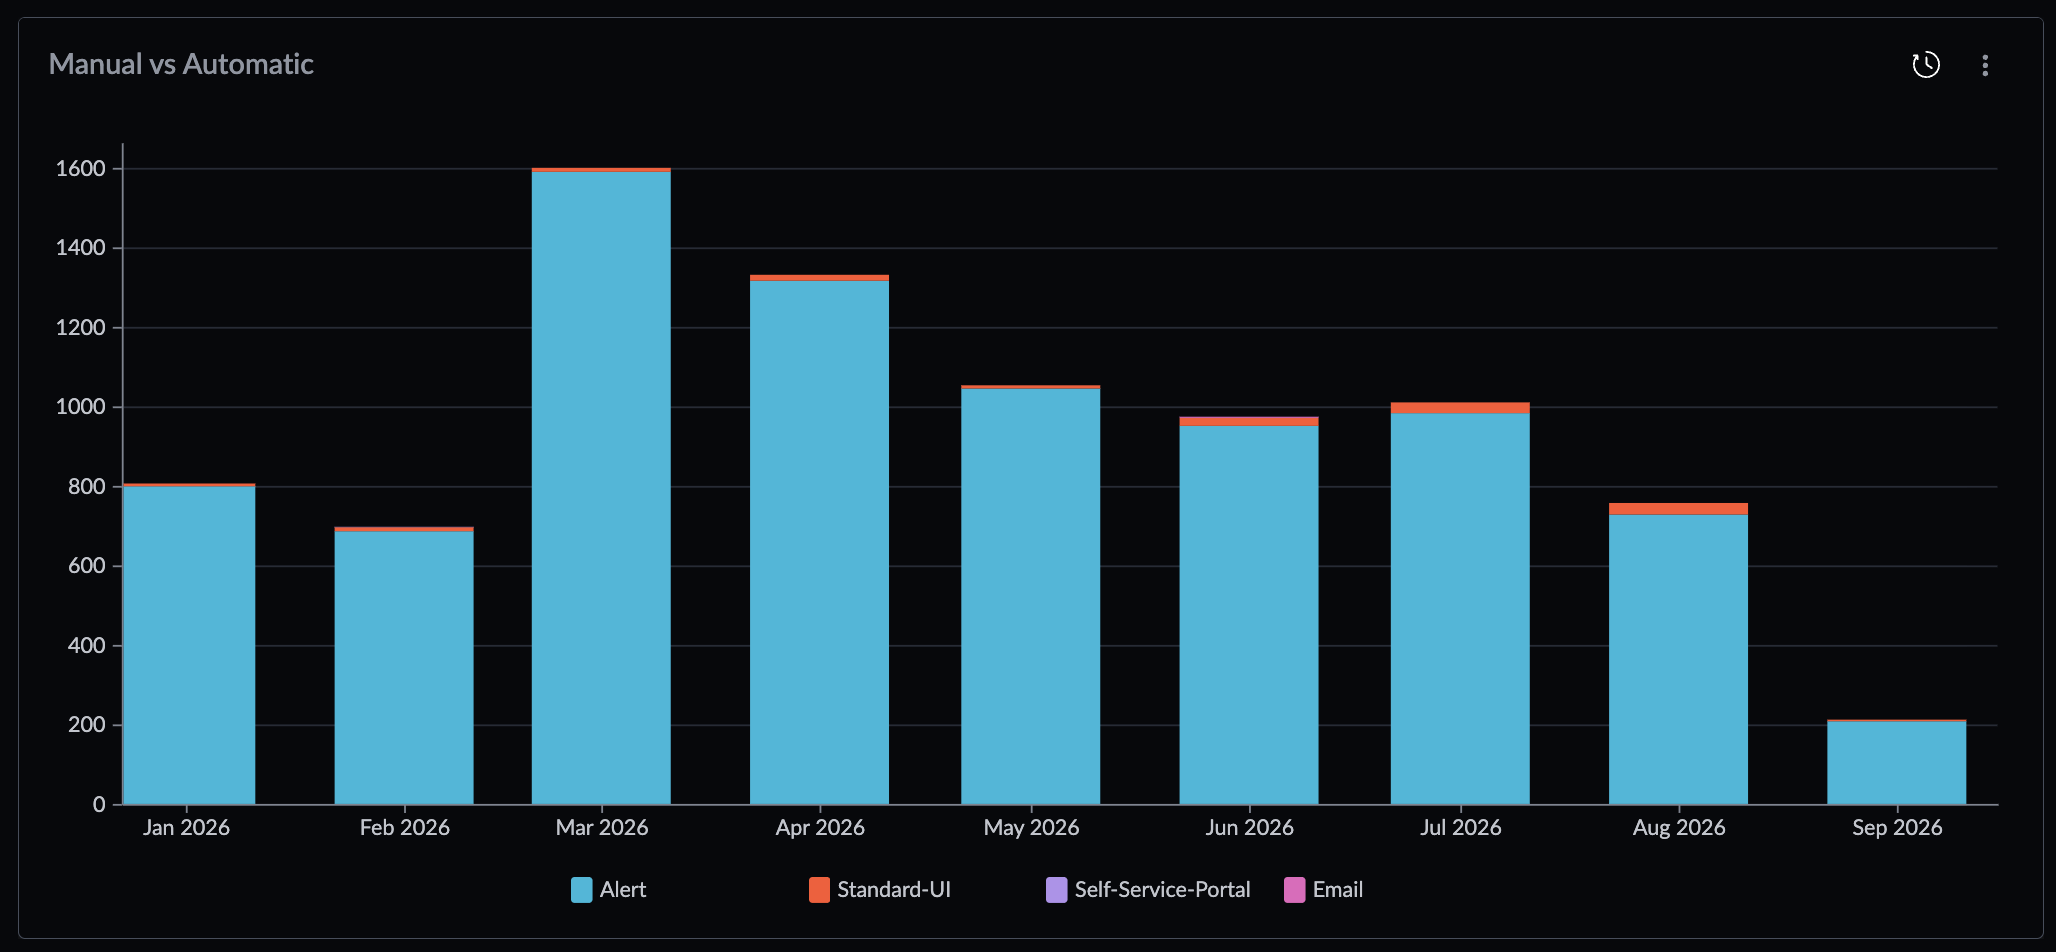
\includegraphics[width=\textwidth,keepaspectratio]{img/itsm_manual_col}
			\caption[Incidentes Manuais vs Automáticos]{Incidentes Manuais vs Automáticos}
			\label{fig:itsm_manual_1}
		\end{figure}
		
		É ainda possível, confirmar na imagem \ref{fig:itsm_manual_2} a quantidade e a percentagem exata de incidentes automáticos (8306 incidentes que corresponde a 98.41\% do \textit{dataset}) e de incidentes manuais (134 incidentes que corresponde a 1.59\% do conjunto de dados).
				
		\begin{figure}[H]
			\centering
			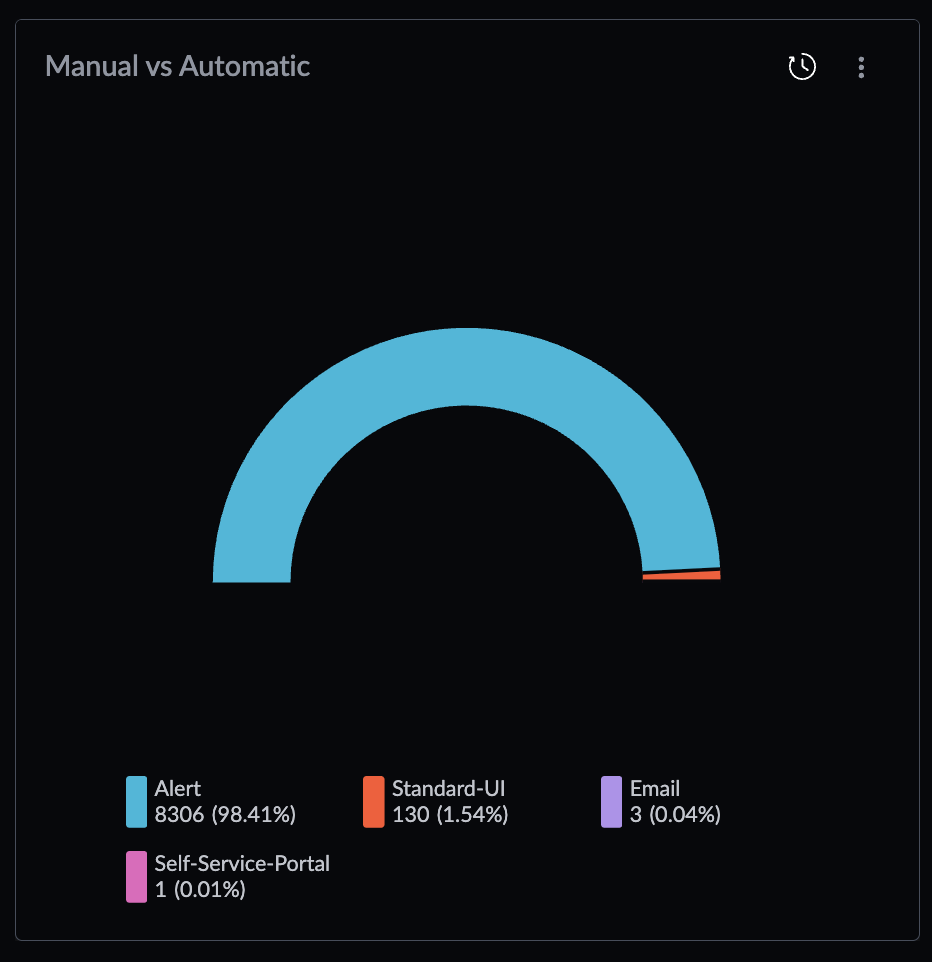
\includegraphics[width=100mm,keepaspectratio]{img/itsm_manual_donut}
			\caption[Percentagem de Incidentes Manuais vs Automáticos]{Percentagem de Incidentes Manuais vs Automáticos}
			\label{fig:itsm_manual_2}
		\end{figure}
		
		Assim, conclui-se que a maioria de dados presentes no \textit{dataset} correspondem a incidentes automáticos que por sua vez têm menos complexidade lexical, uma vez que, para um mesmo problema são gerados com um titulo exatamente similar.
	
%----------------------------------------------------------------------------------------
	\subsection{Destino dos Incidentes}

		Após a criação de um incidente, este pode continuar com a equipa que iniciou a análise ou ser encaminhado para outra equipa, dependendo do tipo de problema ou do serviço afetado. Em ambientes com várias equipas, é comum que a equipa que recebe inicialmente o incidente não tenha o conhecimento necessário para o resolver, sendo necessário direciona-lo para a equipa mais adequada. A atribuição inicial é muitas vezes feita com base no serviço ou na área de negócio afetada, o que nem sempre corresponde à origem técnica do problema.
		
		O encaminhamento de incidentes pode ter impacto direto no tempo necessário para a sua resolução. Quando um incidente é encaminhado para a equipa errada, pode haver perda de tempo, repetição de trabalho e atrasos na investigação, podendo levar a um maior impacto em incidentes críticos. Além disso, decidir para que equipa deve ser encaminhado pode exigir uma análise mais detalhada do incidente e a consulta de casos anteriores. Por isso, mecanismos que ajudem a classificar os incidentes, encontrar casos semelhantes e identificar a equipa mais adequada podem facilitar este processo e reduzir o tempo de resolução.
		
		A análise do ano corrente, presente na imagem \ref{fig:itsm_redirect_1}, demonstra que a maioria dos incidentes não são redirecionados, e que existe uma quantidade reduzida de incidentes reencaminhados uma ou mais vezes.
		
		\begin{figure}[H]
			\centering
			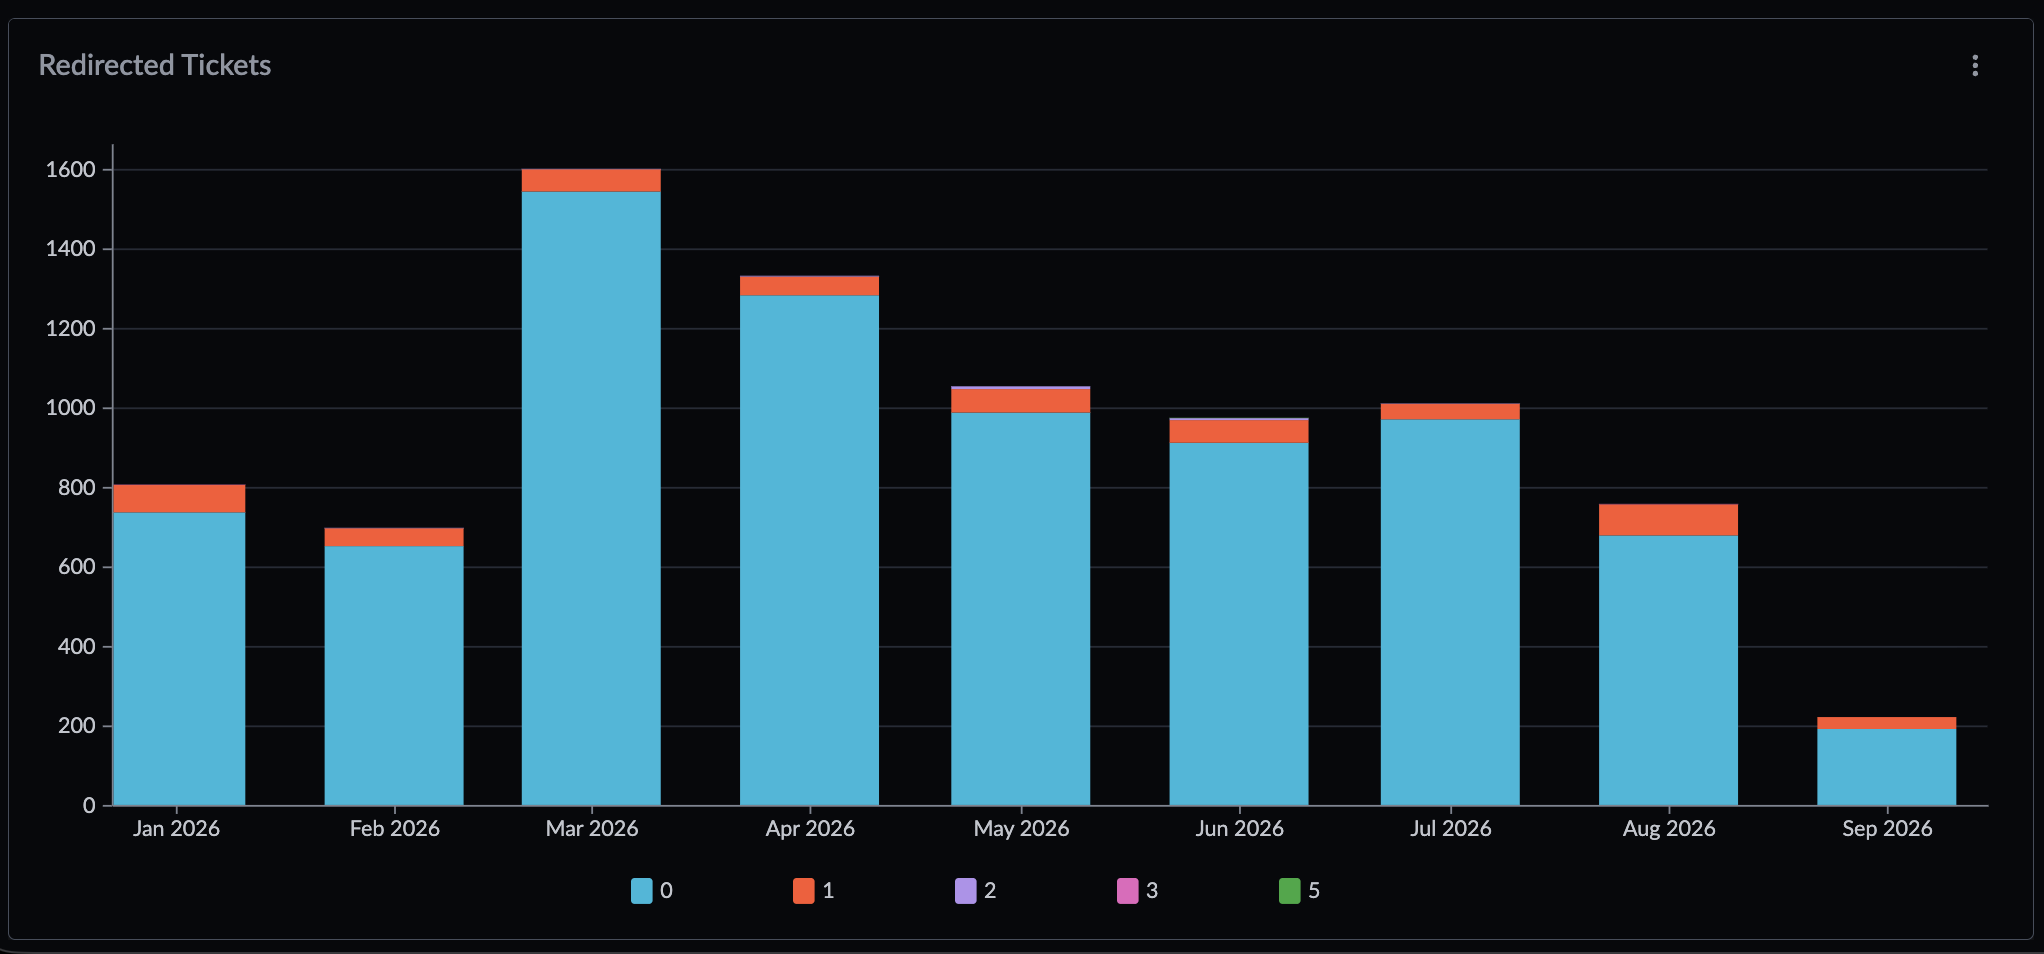
\includegraphics[width=\textwidth,keepaspectratio]{img/itsm_redirect_col}
			\caption[Incidentes Redirecionados]{Incidentes Redirecionados}
			\label{fig:itsm_redirect_1}
		\end{figure}
		
		É ainda possível, confirmar na imagem \ref{fig:itsm_redirect_2} a quantidade e a percentagem exata de incidentes não encaminhados (7949 incidentes que corresponde a 94.08\% do dataset), de incidentes redirecionados apenas uma vez (480 incidentes que corresponde a 5.68\% do conjunto de dados) e os que são reencaminhados mais do que uma vez (20 incidentes correspondentes à quantia restante).
		
		\begin{figure}[H]
			\centering
			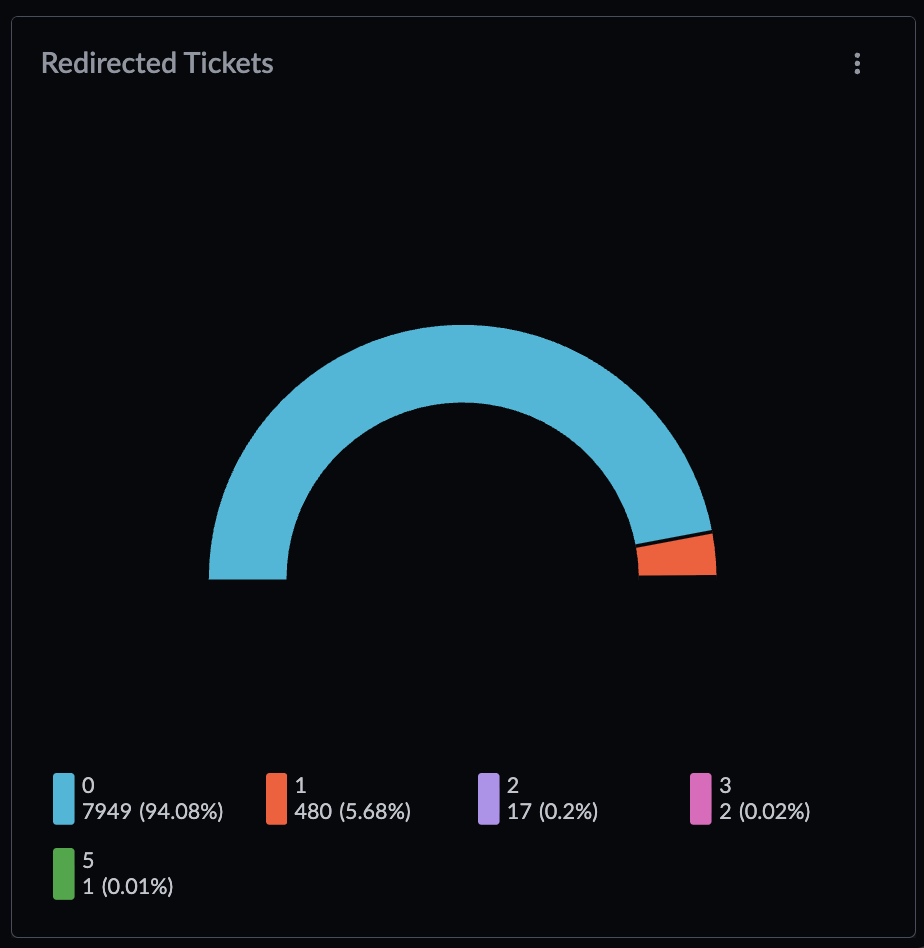
\includegraphics[width=100mm,keepaspectratio]{img/itsm_redirect_donut}
			\caption[Percentagem de Incidentes Redirecionados]{Percentagem de Incidentes Redirecionados}
			\label{fig:itsm_redirect_2}
		\end{figure}
		
		Incidentes reencaminhados duas ou mais vezes, podem indicar maus processos de análise e reencaminhamento, o que pode, novamente, atrasar na resolução de problemas no serviço.
		
		No contexto do produto a ser analisado, a maioria de incidentes não são redirecionados, o que indica que foram atribuidos corretamente, porém este numero pode ser enganador, visto que, normalmente, incidentes automáticos são corretamente encaminhados. Isto significa assim, que apesar do valor de incidentes reencaminhado parecer escasso, analisando apenas o conjunto de registos manuais, estes valores são completamente diferentes, como mostra a imagem \ref{fig:itsm_redirect_manual_1}. 
		
		\begin{figure}[H]
			\centering
			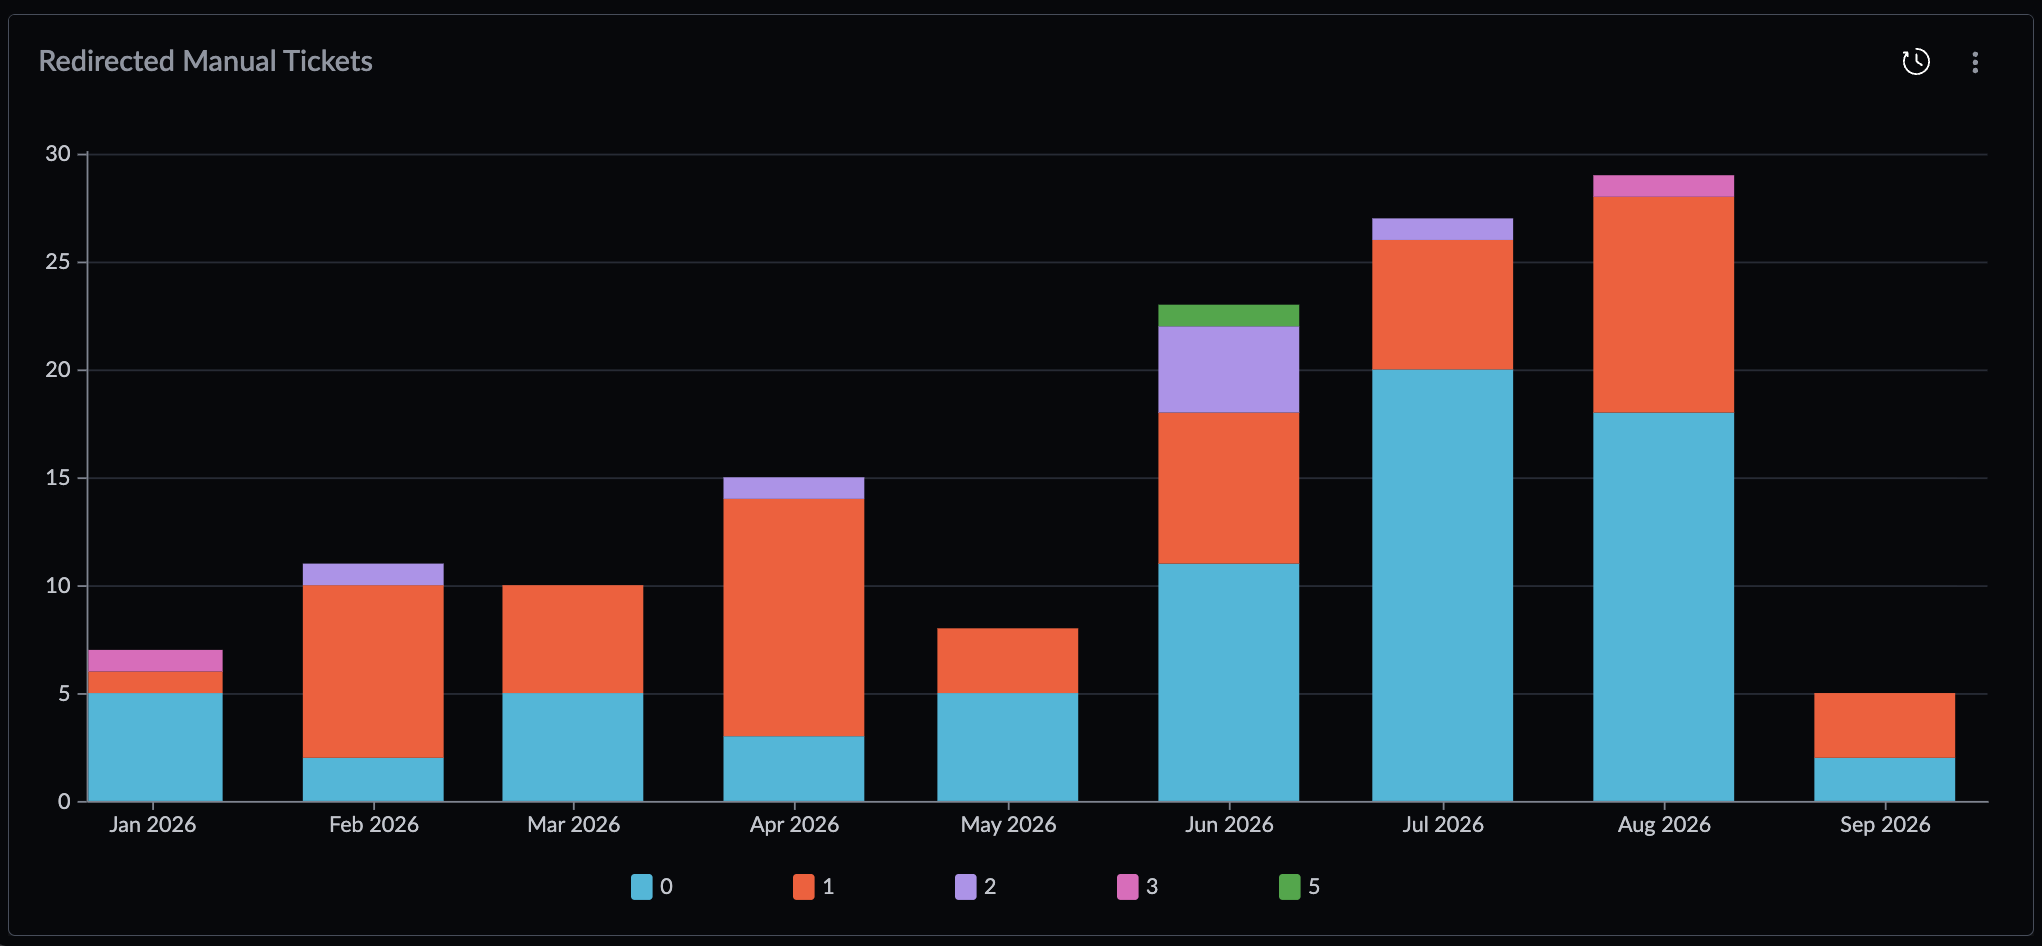
\includegraphics[width=\textwidth,keepaspectratio]{img/itsm_redirect_manual_col}
			\caption[Incidentes Manuais Redirecionados]{Incidentes Manuais Redirecionados}
			\label{fig:itsm_redirect_manual_1}
		\end{figure}
		
		Podemos então confirmar, na imagem \ref{fig:itsm_redirect_manual_2}, que a quantidade de incidentes manuais que são redirecionados é de 47.41\%, sendo assim uma amostra mais significativa.
		
		\begin{figure}[H]
			\centering
			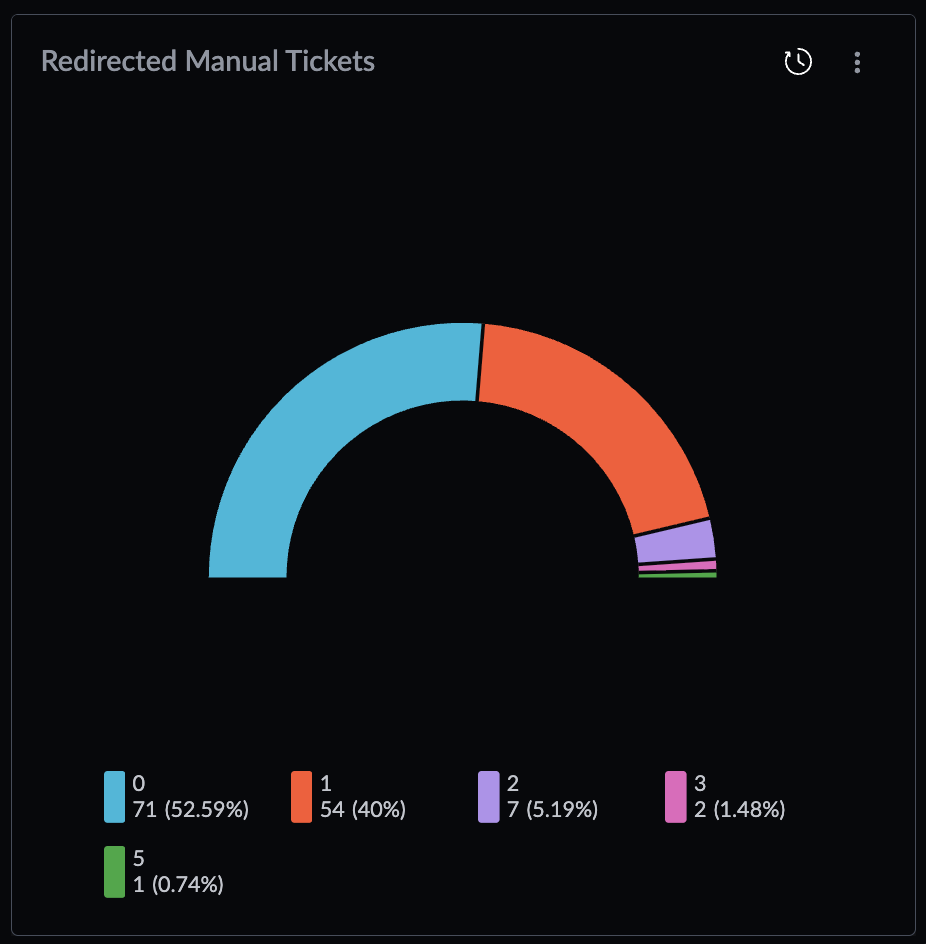
\includegraphics[width=100mm,keepaspectratio]{img/itsm_redirect_manual_donut}
			\caption[Percentagem de Incidentes Manuais Redirecionados]{Percentagem de Incidentes Manuais Redirecionados}
			\label{fig:itsm_redirect_manual_2}
		\end{figure}
		
		Deduz-se portanto, que é importante realizar uma boa análise do incidente, com recurso a histórico e incidentes relacionados, com o objetivo de indicar ao utilizador se o mesmo deve mitigar o problema ou encaminha-lo para a equipa mais competente.
		
%----------------------------------------------------------------------------------------
	\subsection{Conclusão}
		
		A análise do \textit{dataset} permite concluir que o foco inicial da solução deve estar nos incidentes gerados automaticamente, uma vez que representam 98,41\% dos registos analisados. Estes incidentes apresentam normalmente informação mais estruturada e padrões semelhantes, tornando possível utilizar o histórico para identificar problemas recorrentes e apoiar a sua resolução.
		
		Apesar de representarem uma parcela menor do conjunto de dados, os incidentes manuais apresentam maior variabilidade e uma maior necessidade de análise, sendo também mais frequentemente reencaminhados entre equipas. Por este motivo, a solução deverá inicialmente procurar apoiar a resolução dos incidentes automáticos, sem deixar de considerar os incidentes manuais como um caso importante para a análise e evolução futura da solução.

%----------------------------------------------------------------------------------------
\section{Engenharia de Requisitos}

	A engenharia de requisitos é uma etapa importante no desenvolvimento de software, uma vez que permite identificar e definir as principais funcionalidades do serviço e as condições que deve cumprir. Nesta fase são recolhidas e organizadas as necessidades do sistema, servindo posteriormente como base para o seu desenvolvimento e avaliação. Os requisitos podem ser divididos principalmente em requisitos funcionais e não funcionais.

%----------------------------------------------------------------------------------------
	\subsection{Requisitos Funcionais}
	
		Os requisitos funcionais descrevem as funcionalidades que o sistema deve disponibilizar e as ações que deve ser capaz de realizar. No contexto deste projeto, os requisitos estão relacionados principalmente com a receção e análise de incidentes, a procura de incidentes semelhantes, a utilização dessa informação pelo \gls{LLM} e a geração e priorização de sugestões de mitigação, visíveis na tabela \ref{tab:requisitos_funcionais}.
		
		Para definir a prioridade dos requisitos, foi utilizado o método \textit{MoSCoW}, que permite dividir os requisitos em quatro níveis de prioridade:
		
		\begin{itemize}
			\item \textbf{\textit{Must have}} - Essencial para o funcionamento da solução;
			\item \textbf{\textit{Should have}} - Importante mas não impede o funcionamento da solução caso não seja implementado;
			\item \textbf{\textit{Could have}} - Pode ser incluído caso existam recursos e tempo disponíveis;
			\item \textbf{\textit{Won't have}} - Não está nos planos imediatos do projeto, mas pode fazer parte dos planos futuros.
		\end{itemize}
		
		Esta classificação permite definir quais as funcionalidades que devem ser desenvolvidas primeiro e ajuda a manter o foco nos objetivos principais da solução.
	
		\begin{table}[H]
			\centering
			\begin{tabular}{p{2.1cm}p{9cm}p{2cm}}
				\hline
				\textbf{Identificador} & \textbf{Descrição} & \textbf{Prioridade} \\
				\hline
				\textit{RF-01} & O sistema deve permitir receber um incidente para análise através do serviço de incidentes. & Must have \\
				\hline
				\textit{RF-02} & O sistema deve obter os dados relevantes do incidente, incluindo a descrição, serviço afetado, severidade e outros campos disponíveis. & Must have \\
				\hline
				\textit{RF-03} & O sistema deve procurar no histórico por incidentes relacionados com o incidente recebido. & Must have \\
				\hline
				\textit{RF-04} & O sistema deve utilizar os incidentes relacionados como contexto para a análise realizada pelo \gls{LLM}. & Must have \\
				\hline
				\textit{RF-05} & O sistema deve gerar um resumo do incidente em linguagem natural. & Must have \\
				\hline
				\textit{RF-06} & O sistema deve gerar sugestões de mitigação com base na informação disponível e nos incidentes relacionados. & Must have \\
				\hline
				\textit{RF-07} & O sistema deve ordenar as sugestões de mitigação de acordo com a sua relevância. & Must have \\
				\hline
				\textit{RF-08} & O sistema deve apresentar a informação utilizada para suportar as sugestões geradas, permitindo consultar os incidentes relacionados. & Must have \\
				\hline
				\textit{RF-09} & O sistema deve permitir identificar a equipa mais adequada para tratar o incidente, quando essa informação fizer parte do objetivo da solução. & Should have \\
				\hline
				\textit{RF-10} & O sistema deve permitir configurar a utilização, ou não, de comentários e notas de análise dos incidentes. & Should have \\
				\hline
				\textit{RF-11} & O sistema deve permitir configurar o modelo utilizado pela \gls{LLM}. & Could have \\
				\hline
				\textit{RF-12} & O sistema deve procurar informação relevante na documentação do serviço afetado, resumir o conteúdo encontrado e utiliza-lo na análise do incidente. & Could have \\
				\hline
				\textit{RF-13} & O sistema deve consultar os logs do serviço afetado para encontrar informação relacionada com o incidente e utilizá-la na análise. & Won't have \\
				\hline
			\end{tabular}
			\caption[Requisitos Funcionais]{Requisitos Funcionais}
			\label{tab:requisitos_funcionais}
		\end{table}
	
%----------------------------------------------------------------------------------------
	\subsection{Requisitos Não Funcionais}

		Os requisitos não funcionais definem características que o sistema deve cumprir, mas que não estão diretamente relacionadas com uma funcionalidade específica. São, normalmente, considerados aspetos como o desempenho, a segurança, a fiabilidade e manutenção da solução, tal como os definidos na tabela \ref{tab:requisitos_nao_funcionais}. Estes requisitos são importantes para garantir que o sistema não só funciona corretamente, mas que também pode ser utilizado de forma adequada num ambiente real.

		\begin{table}[H]
			\centering
			\begin{tabular}{p{2.2cm}p{11cm}}
				\hline
				\textbf{Identificador} & \textbf{Descrição} \\
				\hline
				\textit{RNF-01} & O sistema não deve expor informação confidencial dos incidentes a utilizadores ou serviços que não tenham autorização para a consultar. \\
				\hline
				\textit{RNF-02} & O sistema deve estar organizado de forma a permitir adicionar, substituir ou remover serviços externos sem impacto no restante serviço. \\
				\hline
				\textit{RNF-03} & O sistema deve limitar a quantidade de informação enviada para o \gls{LLM}, de forma a manter o custo de cada análise dentro de valores aceitáveis. \\
				\hline
			\end{tabular}
			\caption[Requisitos não Funcionais]{Requisitos não Funcionais}
			\label{tab:requisitos_nao_funcionais}
		\end{table}
	
\section{Desenho}
	
	Como referido anteriormente, o objetivo da solução passa por integrar com diversos serviços externos, tais como:
	\begin{itemize}
		\item \textbf{Serviço de incidentes:} apresenta-se como sendo a base da solução, é a partir deste serviço que retiramos a informação do incidente a ser analisado e do histórico de incidentes, para realizar a correlação;
		\item \textbf{Serviço de documentação:} com informação retirada do incidente, fornece documentação do serviço afetado;
		\item \textbf{Motor \gls{LLM}:} outro elemento que devemos considerar como base da solução, visto que é responsável por fazer a ligação entre o incidente principal, os incidentes relacionados e a documentação do serviço devolvendo um resumo em linguagem natural e as sugestões de mitigação priorizarizadas.
	\end{itemize}
	
	Assim, a solução proposta combina a informação obtida do serviço de incidentes e documentação com as capacidades de análise do motor \gls{LLM}. Esta combinação permite analisar o incidente atual com base no histórico disponível, gerar uma descrição em linguagem natural e apresentar sugestões de mitigação.
	
%----------------------------------------------------------------------------------------
	\subsection{Diagrama de Implantação}
	
	Para além dos serviços funcionais descritos, a solução proposta deve, futuramente, ser exposta através de uma interface de acesso controlada e escalável. Desta forma, propomos a utilização de um \textit{API Gateway} (Gateway de API) para agir como uma porta de entrada do serviço, controlando autorizações e acessos, e gerir o tráfego de pedidos feitos à \gls{API}. Em paralelo, apresentamos a necessidade de um \textit{Load Balancer} (balanceador de carga) que ajuda a distribuir tráfego entre múltiplas instâncias do serviço, assegurando maior disponibilidade e tolerância a falhas.
	
	Adicionalmente, é sugerido o desenvolvimento de uma aplicação \textit{Web} que permita a visualização da informação gerada por parte dos \gls{OCEs}, onde estes poderão consultar o resumo do incidente pretendido, \textit{tickets} relacionados e sugestões de mitigação.
	
	\begin{figure}[H]
		\centering
		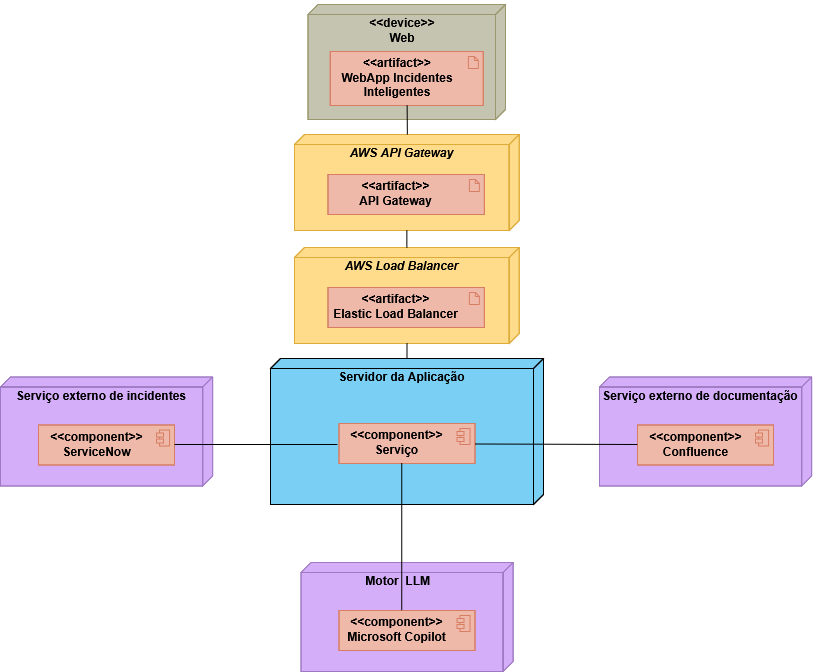
\includegraphics[width=110mm,keepaspectratio]{img/diagramaDeployment_v3}
		\caption[Diagrama de Implantação]{Diagrama de Implantação}
		\label{fig:deployDiagram}
	\end{figure}
	
	%----------------------------------------------------------------------------------------
	\subsection{Diagrama de Sequência}
	
	O diagrama de sequência apresentado na Figura \ref{fig:sequenceDiagram}, representa um fluxo bem sucedido de recuperação e enriquecimento de contexto utilizado na análise de um incidente. O processo começa com a obtenção dos dados do incidente, através do serviço de \textit{ITSM}. De seguida, é realizada uma primeira chamada ao \gls{LLM}, utilizando a informação do incidente e tem como objetivo identificar possíveis incidentes relacionados e o serviço afetado.
	
	Com base no serviço identificado, o sistema pesquisa as páginas disponíveis no espaço definido do \textit{Confluence} e obtém o conteúdo de cada uma. Para cada página encontrada, é realizada uma chamada ao \gls{LLM}, onde o modelo avalia se o conteúdo da página é relevante para o incidente em análise. Este processo é repetido até que todas as páginas obtidas sejam verificadas. Desta forma, cada página é analisada individualmente com base no contexto do incidente, de forma, a que o modelo não crie alucinações.
	
	De seguida, o sistema pesquisa no \textit{ITSM} outros incidentes com o mesmo título do incidente em análise, mantendo apenas os dados considerados relevantes. Os incidentes relacionados identificados na primeira etapa são também obtidos e combinados com a restante informação recolhida.
	
	Por fim, o incidente original, os incidentes relacionados, os incidentes com o mesmo título e as páginas consideradas relevantes são enviados numa chamada final ao \gls{LLM}. Esta chamada utiliza todo o contexto recolhido para produzir o resumo do incidente e as respetivas sugestões de mitigação.
	
	\begin{figure}[H]
		\centering
		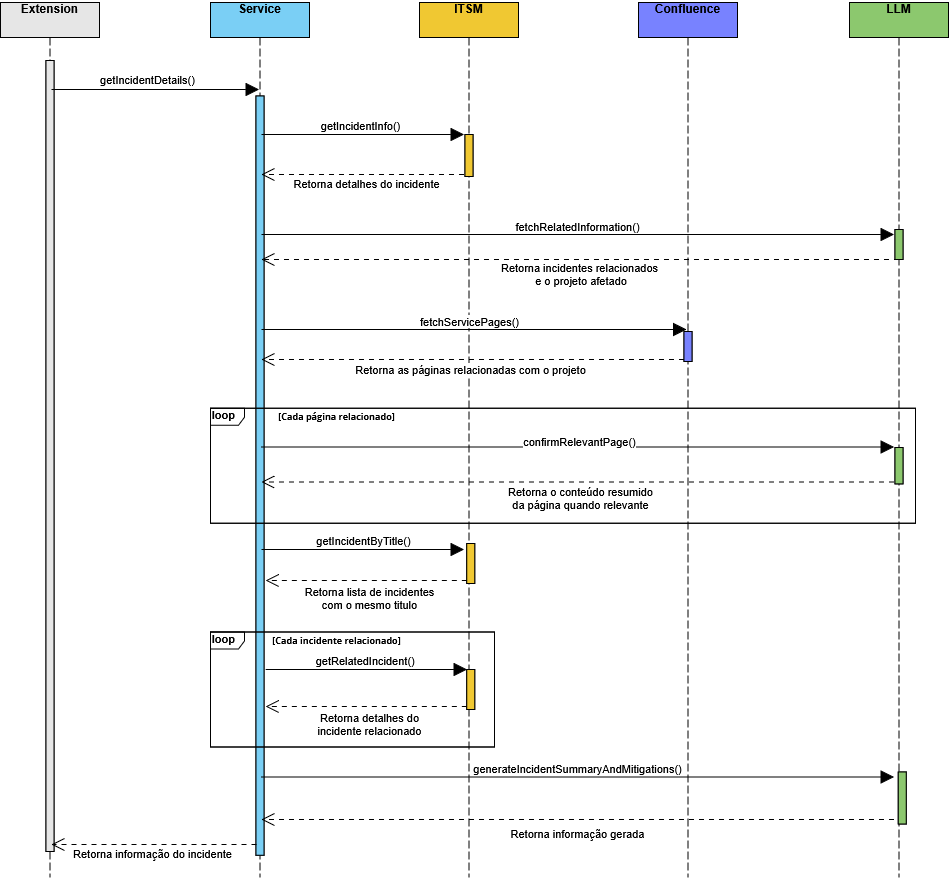
\includegraphics[width=\textwidth,keepaspectratio]{img/diagramaSequencia_v4}
		\caption[Diagrama de Sequência]{Diagrama de Sequência}
		\label{fig:sequenceDiagram}
	\end{figure}

%----------------------------------------------------------------------------------------
\section{Conclusão}

	Neste capítulo observamos o planeamento da solução desenvolvida, sendo apresentadas as funcionalidades principais e as integrações externas. Além disso, abordaram-se estatísticas sobre o conjunto de dados que permitem perceber qual a maior área de impacto do serviço. Por fim, apresentaram-se requisitos que descrevem as principais funcionalidades e características do sistema a serem desenvolvidas e os diagramas que permitem ter uma visão do fluxo de cada análise de incidente.